\section{Problem and domain analysis}
\phantomsection

\subsection{Indexes}

A database index is a data structure that improves the speed of data retrieval operations on a database table at the cost of additional writes and storage space to maintain the index data structure. Indexes are used to quickly locate data without having to search every row in a database table every time a database table is accessed. Indexes can be created using one or more columns of a database table, providing the basis for both rapid random lookups and efficient access of ordered records.

An index is a copy of selected columns of data from a table that can be searched very efficiently that also includes a low-level disk block address or direct link to the complete row of data it was copied from. Some databases extend the power of indexing by letting developers create indexes on functions or expressions. 

\subsection{Indexes Usage}
\subsubsection{Support for fast lookup}
Most database software includes indexing technology that enables sub-linear time lookup to improve performance, as linear search is inefficient for large databases.

Suppose a database contains N data items and one must be retrieved based on the value of one of the fields. A simple implementation retrieves and examines each item according to the test. If there is only one matching item, this can stop when it finds that single item, but if there are multiple matches, it must test everything. This means that the number of operations in the worst case is O(N) or linear time. Since databases may contain many objects, and since lookup is a common operation, it is often desirable to improve performance.

An index is any data structure that improves the performance of lookup. There are many different data structures used for this purpose. There are complex design trade-offs involving lookup performance, index size, and index update performance. Many index designs exhibit logarithmic (O(log(N))) lookup performance and in some applications it is possible to achieve flat (O(1)) performance.

\subsubsection{Policing the database constraints}
Indexes are used to police database constraints, such as UNIQUE, EXCLUSION, PRIMARY KEY and FOREIGN KEY. An index may be declared as UNIQUE, which creates an implicit constraint on the underlying table. Database systems usually implicitly create an index on a set of columns declared PRIMARY KEY, and some are capable of using an already existing index to police this constraint. Many database systems require that both referencing and referenced sets of columns in a FOREIGN KEY constraint are indexed, thus improving performance of inserts, updates and deletes to the tables participating in the constraint.

Some database systems support an EXCLUSION constraint that ensures that, for a newly inserted or updated record, a certain predicate holds for no other record. This can be used to implement a UNIQUE constraint (with equality predicate) or more complex constraints, like ensuring that no overlapping time ranges or no intersecting geometry objects would be stored in the table. An index supporting fast searching for records satisfying the predicate is required to police such a constraint.

\subsection{Index architecture/Indexing Methods}

\subsubsection{Clustered}
Clustering alters the data block into a certain distinct order to match the index, resulting in the row data being stored in order. Therefore, only one clustered index can be created on a given database table. Clustered indices can greatly increase overall speed of retrieval, but usually only where the data is accessed sequentially in the same or reverse order of the clustered index, or when a range of items is selected.

Since the physical records are in this sort order on disk, the next row item in the sequence is immediately before or after the last one, and so fewer data block reads are required. The primary feature of a clustered index is therefore the ordering of the physical data rows in accordance with the index blocks that point to them. Some databases separate the data and index blocks into separate files, others put two completely different data blocks within the same physical file(s).

\subsubsection{Non-clustered}
The data is present in arbitrary order, but the logical ordering is specified by the index. The data rows may be spread throughout the table regardless of the value of the indexed column or expression. The non-clustered index tree contains the index keys in sorted order, with the leaf level of the index containing the pointer to the record (page and the row number in the data page in page-organized engines; row offset in file-organized engines).

In a non-clustered index,

The physical order of the rows is not the same as the index order.
The indexed columns are typically non-primary key columns used in JOIN, WHERE, and ORDER BY clauses.
There can be more than one non-clustered index on a database table.

\subsection{MSSQL Execution Plan}
A query plan, execution plan, or query execution plan is an algorithm showing a set of steps in a specific order that is executed to access data in a database

A query plan shows how a query was executed, or how it will be executed which is significant for troubleshooting query performance issues. Executing a SELECT statement to find out its query plan and effect on SQL Server performance can be acceptable, but executing UPDATEs to find that out is not an option. The plan is calculated by a SQL Server component Query Optimizer using minimum of server resources. When creating the SQL Server query execution plan, the number of database objects involved, joins, indexes and their availability, number of output columns, and more is considered

When a new query is executed, Query Optimizer evaluates the query plan, optimizes and compiles it, and stores it in the plan cache. The plan cache is a part of SQL Server buffer where data and query plans are stored (buffered), so they can be reused later

When a query is executed, Query Optimizer first searches the plan cache looking for a query plan that can be reused, thus making the execution faster. If there’s no query plan that can be reused, a new one has to be created, which takes time and therefore makes query execution last longer

A very useful characteristic of query plans is that when a stored procedure is executed, the query plan is created for the stored procedure name and the same query plan will be reused whenever the stored procedure is executed, despite the values specified for procedure parameters. When it comes to executing ad hoc queries, query plans are created based on complete code, so different parameters or any change in code will prevent reuse of the existing plan. This clearly indicates what should be done to make your code run faster – wrap it up as stored procedures or functions, and the existing query plans will be reused and therefore code will be executed much faster

The slow execution of ad hoc queries can be mitigated by using the Optimize for ad hoc workloads option, introduced in SQL Server 2008. The option optimizes the plan cache use, as it solves the situation when query plans executed only once fill up the plan cache. As the buffer cache is used for both data and plan buffering, and the percentage of cache used for each changes in time depending on the current situation, it’s necessary to use the cache wisely. Instead of buffering the whole plan, when the option is set to “True”, only a fragment of the plan is buffered when the query is executed for the first time. When an ad hoc query is executed for the second time, its complete plan is buffered in the cache


\subsection{MSSQL Execution Plan Elements}
Since we are using Indexes for optimization of database, we need to know great tools given by Microsoft like Execution Plan. Execution Plan tells us what happens behind of query, what operations are done,what cost has every operations and how are merged together. We will use this functionality for analyzing effects of Indexation. 
\\
Although execution plan has a lot of elements, in this course work we will cover only few definitions such as Scan,Seek and types of Joins. 

\subsubsection{Scan}
Since a scan touches every row in the table, whether or not it qualifies, the cost is proportional to the total number of rows in the table. Thus, a scan is an efficient strategy if the table is small or if most of the rows qualify for the predicate.
\begin{figure}[ht!]
	\centering
	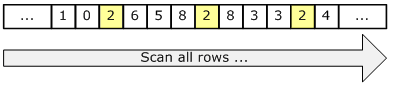
\includegraphics[width=0.6\textwidth]{scan}
	\caption{Scan algorithm}
\end{figure}

\subsubsection{Seek}
Since a seek only touches rows that qualify and pages that contain these qualifying rows, the cost is proportional to the number of qualifying rows and pages rather than to the total number of rows in the table.

Index Scan is nothing but scanning on the data pages from the first page to the last page. If there is an index on a table, and if the query is touching a larger amount of data, which means the query is retrieving more than 50 percent or 90 percent of the data, and then the optimizer would just scan all the data pages to retrieve the data rows. If there is no index, then you might see a Table Scan (Index Scan) in the execution plan.

Index seeks are generally preferred for the highly selective queries. What that means is that the query is just requesting a fewer number of rows or just retrieving the other 10 (some documents says 15 percent) of the rows of the table.
\begin{figure}[ht!]
	\centering
	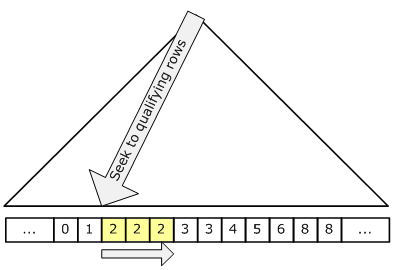
\includegraphics[width=0.6\textwidth]{seek}
	\caption{Seek algorithm}
\end{figure}

\subsubsection{SQL Joins \cite{SQLJoins}}
SQL Server employs three types of join operations:

\begin{itemize}	
	\item Nested loops joins
	\item Merge joins
	\item Hash joins
\end{itemize}

If one join input is small (fewer than 10 rows) and the other join input is fairly large and indexed on its join columns, an index nested loops join is the fastest join operation because they require the least I/O and the fewest comparisons. For more information about nested loops, see Understanding Nested Loops Joins.

If the two join inputs are not small but are sorted on their join column (for example, if they were obtained by scanning sorted indexes), a merge join is the fastest join operation. If both join inputs are large and the two inputs are of similar sizes, a merge join with prior sorting and a hash join offer similar performance. However, hash join operations are often much faster if the two input sizes differ significantly from each other. For more information, see Understanding Merge Joins.

Hash joins can efficiently process large, unsorted, non indexed inputs.
\\
For examples we can look into \cite{Joins}.

\subsection{Problem definition}
Main scope of this course work is to demonstrate indexation and it's benefits.So we will divide our problem into two parts.
\begin{itemize}
	\item Clustered Index
	\item Non Clustered Index
\end{itemize}
Both subproblems will have their own purpose and own examples. Each subproblem has an definition,analysis,solution and post-analysis. 

\clearpage